\documentclass[11pt,a4paper]{article}
\usepackage[utf8]{inputenc}
\usepackage[german]{babel}
\usepackage{amsmath}
\usepackage{amsfonts}
\usepackage{hyperref}
\usepackage{booktabs}
\usepackage{setspace}
\usepackage{threeparttable}
\usepackage{amssymb}
\usepackage{graphicx}
\usepackage{fancyhdr}
\usepackage{icomma}
\usepackage{float}
\usepackage{pdfpages}
\usepackage{hyperref}
\usepackage[left=2.5cm,right=2.5cm,top=2cm,bottom=3.5cm]{geometry}
\usepackage{csquotes}
\title{DreamSwipe\\Tinder für Filme\vspace{10px}}
\author{Leon Gieringer, Robin Meckler,Vincent Schreck \\ \\ Studienarbeit \\ \\ \\}
\date{\today}

\begin{document}
\maketitle
\thispagestyle{empty}
\newpage
\pagenumbering{Roman}
\tableofcontents
\newpage
\pagenumbering{arabic}

\pagestyle{fancy}
\fancyhf{}
\setlength{\headheight}{35pt}
\lhead{DreamSwipe}
\rhead{Studienarbeit}
\cfoot{\thepage}
\newpage


\section{Einleitung}


\section{Motivation}


\section{Theoretische Grundlagen}


\subsection{Anwendungsentwicklung für mobile Endgeräte}
\label{sec:mobile_development}
Mobile Geräte sind heutzutage ein sehr großer Teil unseres Tagesablaufs. Durchschnittlich verbringen wir 3:54 Stunden pro Tag an mobilen Geräten (hier bezogen aus Bürger der USA). Die meiste Zeit hiervon wird in Apps (ca. 90\%). \footnote{\url{https://www.emarketer.com/content/us-time-spent-with-mobile-2019}, zuletzt aufgerufen: 26.02.2021} 
Laut Cisco wird dieser Markt sich jedoch nicht nur auf Industrieländer beruhen, sondern bis 2023 sollen weltweit 71\% der Bevölkerung mobile Konnektivität haben. \cite{cisco2020}
Diese Entwicklung forcierte viele Firmen immer mehr ihre Anwendungen auch \textit{mobile ready} zu gestalten. Dies kann man bspw. deutlich bei der Anpassung vieler Webseiten an Mobile Seiten- und Größenverhältnisse oder auch dem Anbieten von \textit{Apps}, welche bereits für Desktop o.ä. verfügbar waren, erkennen. \\

Daher ist es für die Wirtschaft und Entwicklung gleichermaßen wichtig sich ständig weiterzuentwickeln und sich nicht auf (Kosten-) ineffiziente Entwicklungsprozesse auszuruhen. Dabei bieten jährliche, wenn nicht sogar halbjährliche Design- und Performanceänderungen von den Geräten selbst oder der Betriebssysteme Herausforderungen an die mobilen Anwendungen - \textit{apps} - und gleichzeitig an deren Programmierumgebung. Trotz einer riesigen Auswahl an \textit{Apps} lassen sich diese allgemein in drei Kategorien eingliedern: Plattformspezifische native Anwendungen, adaptive Webanwendungen und plattformübergreifende Anwendungen.

\subsubsection{Begriffe}
\subparagraph{Eine Plattform} besteht aus der Hardware (System und zusätzlicher Peripherie, wie Sensoren oder Aktoren), dem Betriebssystem, den spezifischen \textit{Software Development Kits (SDK)} und den jeweiligen Basisbibliotheken. 
Zusammen bietet eine Plattform die Grundlage um Software für sie zu entwickeln.
\subparagraph{Ein \textit{Framework}} definiert eine Architektur für Anwendungen und stellt Komponenten bereit, mit welchen das Entwickeln einer Anwendung erleichtert sein soll. \cite{johnson1988} 
Ein plattformübergreifendes Framework muss somit Anwendungscode für mehrere Plattformen wiederverwenden, jedoch müssen auch plattformspezifische Funktionen, wie Architektur oder Benutzeroberflächen API, bereitgestellt werden. Mehr dazu in Kapitel \ref{plattformuebergreifende_anwendungen}.

\subparagraph{Eine mobile Anwendung} ist eine Anwendung, geschrieben für eine Plattform eines mobilen Endgerätes, welche die jeweiligen Features nutzen könnte - dazu zählen Kamera(s), Beschleunigungssensoren oder auch \textit{Global Positioning System (GPS)}. Webseiten als solches sind demnach keine mobilen Anwendungen.


\subsubsection{Plattformspezifische native Apps}
Plattformspezifische oder auch native Anwendungen sind Programme, welche auf eine gewisse Plattform abzielen und in einer der davon unterstützen Programmiersprachen geschrieben wurden. Da diese Art der (mobilen) Anwendung mit plattformspezifischen  SDK und \textit{Frameworks} entwickelt wird, ist diese Anwendung an eine Plattform gebunden. \\
Dies bringt zum einen natürlich Vorteile wie allgemein best mögliche Performance auf der jeweiligen Plattform und direkt vom Hersteller unterstützte Entwicklungsumgebungen/SDKs.
Zudem lassen sich plattformspezifische Fähigkeiten oder Einstellungen nutzen - beispielsweise mehrere Kameras oder GPS.

Gleichzeitig beschränkt man sich aber logischerweise auf eine Plattform und deckt mit einer Anwendung nur einen Teil des gesamten Marktes. Dies bringt im Vergleich zu den anderen Möglichkeiten einen deutlich erhöhten Entwicklungs- und Wartungsaufwand mit sich, da für andere Plattformen Programmcode nicht übernommen werden kann. Zusätzlich benötigen Entwickler spezifische Kompetenzen für beide Plattform und Entwicklungsumgebungen. \\

Zwei der am weitesten verbreiteten Plattformen sind Android von Google und iOS von Apple. Anwendungen für Android können in Kotlin oder Java als Programmiersprache beispielsweise in dem \textit{integrated development environment (IDE)} von Google Android Studio entwickelt werden. Für iOS wird hingegen mit Objective-C und Swift als Programmiersprache primär in der IDE XCode entwickelt.

Beide bieten jeweils Plattform eigene Services an, beispielsweise das direkte Veröffentlichen in den jeweiligen Appstore \cite{fentaw2020}

\subsubsection{Plattformübergreifende Anwendungen}
\label{plattformuebergreifende_anwendungen}
Die Entwicklung einer plattformübergreifenden Anwendung zeichnet sich generell durch die Möglichkeit aus, nur einmal Code schreiben zu müssen, diesen jedoch auf mehreren Plattformen ausführen zu können. \\
Verschiedene Ansätze einer solchen Anwendung sind in Abbildung \ref{fig:crossplattform_architecture} kategorisiert. Im Folgenden werden jene Entwicklungsmöglichkeiten detaillierter besprochen.

\begin{figure}[h]
	\begin{center}
		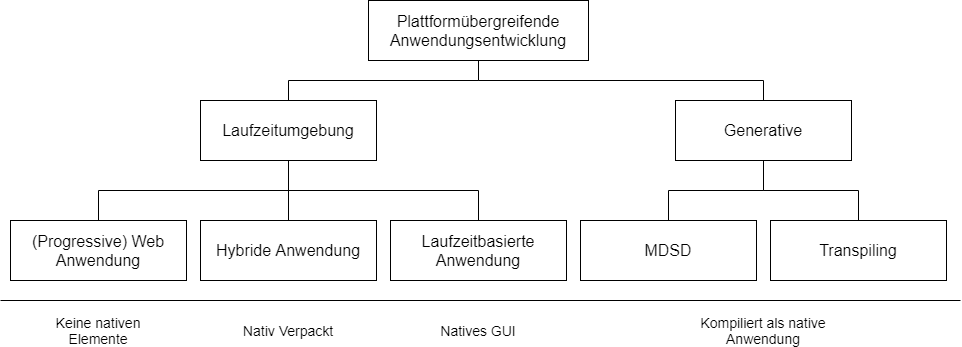
\includegraphics[scale=0.47]{images/crossplattform_unterteilung.png}
	\end{center}
	\caption{Kategorisierung verschiedener plattformübergreifender Ansätze. Erstellt nach \cite{majchrzak2015} \protect}
	\label{fig:crossplattform_architecture}
\end{figure}

\paragraph{\textit{(Progressive) Web Apps}}
Eine mobile Webanwendung ist eigentlich eine Webseite, welche sich an die Größe und Auflösung von unterschiedlichen Bildschirmen anpasst - hier speziell an die Bildschirmgrößen der mobilen Geräte. Diese Anwendung ist mit Standard Webentwicklungstools geschrieben (HTML, CSS \& JavaScript) und läuft somit theoretisch auf jedem Gerät mit einem Internet Browser. \cite{charland2011}
Aufgrund der steigenden Unterstützung von jeglichen APIs in mobilen Browsern, ist es auch möglich geworden auf Geräteeigenschaften, wie bspw. den Standort zuzugreifen.\\
Jedoch kann diese App logischerweise nicht im jeweiligen \textit{Appstore} heruntergeladen werden, da es sich weiterhin um eine Webseite handelt.
Aus gleichem Grund kann hiermit auch kein \glqq natives Design und Leistung\grqq erzeugt werden.\\

Abhilfe hierfür sorgt jedoch die von Google vorgestellte Design Idee \textit{Progressive Web Apps} (PWA). Sie bietet die Möglichkeit Code in sog. \textit{service worker} als Hintergrundthread ausführen zu lassen, ein Webseiten Manifest anzugeben, die App offline bedienen zu können und bieten die Möglichkeit die PWA zu installieren. Gleichzeitig kann mit diesem Design eine zu nativen Apps vergleichbare Leistung erreicht werden.\cite{bjorn-hansen2020} \\

Generell ist der Ansatz sehr simpel, da hiermit plattformübergreifende Anwendungen geschrieben werden können, welche sich auf allen Geräten mit Browser bedienen lassen. 
Hierfür wird zudem keine zusätzliche Programmiersprache oder wissen über die jeweilige Plattform benötigt.\\
Eine große Schwierigkeit hieran ist weiterhin der Zugriff auf Gerätefeatures, da nicht alle über den Browser verfügbar sind.

\paragraph{Hybride Anwendungen}
\label{hybride_anwendung}
Eine hybride Anwendung kombiniert die native Vorgehensweise mit der einer normalen Webseite. 
In einer nativen WebView ist eine Webanwendung verpackt, welche nun in einer \textit{HTML-Rendering-Engine} gerendert wird. Bei Android und iOS ist das WebKit.
Diese WebView funktioniert ähnlich wie ein normaler Browser, jedoch werden Kontrollfenster nicht angezeigt, wie zum Beispiel Adresszeile, Einstellungen oder Lesezeichen.
Ähnlich wie bei Web Anwendungen werden über JavaScript APIs Gerätefeatures eingebunden.\\
Ein sehr frühes Framework für diese Art von Anwendung war \href{https://cordova.apache.org/}{Adobe Cordova}, eher bekannt als das ursprüngliche PhoneGap von Nitobi. Viele weitere Frameworks basieren auf ihren Anfängen.\\

Eine hybride Anwendung kann also normal als App im \textit{Appstore} heruntergeladen auf dem Gerät installiert und offline genutzt werden - also sehr ähnlich zu nativen Lösungen. Daher ist dieser Ansatz auch sehr beliebt 
Daher liegt auch hier die Leitung der Applikation deutlich hinter der der Nativen. \cite{lachgar2017} \cite{bjorn-hansen2020}

\begin{figure}[tbt]
	\begin{center}
		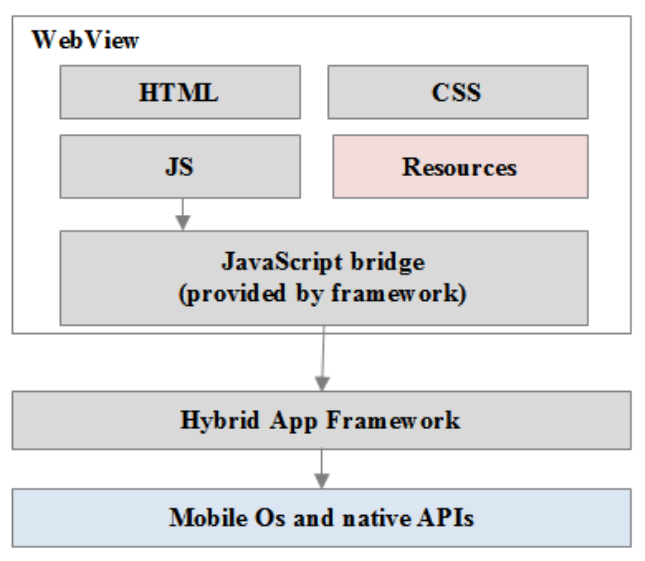
\includegraphics[scale=0.45]{images/hybride-anwendungen-struktur.PNG}
	\end{center}
	\caption{Struktur einer hybriden Anwendung \protect \footnotemark}
	\label{fig:hybrid_structure}
\end{figure}
\footnotetext{Quelle: \cite{lachgar2017}}

\paragraph{Runtime basierte Anwendungen}
\label{runtime_based_apps}
Im Gegensatz zur in Kapitel \ref{hybride_anwendung} beschriebenen hybriden Anwendung, nutzen Runtime basierte Anwendungen keinen Browser des Gerätes mit einer WebView, sondern jede App besitzt eine eigene Runtime Ebene. 
Jedes Framework muss also eine solche Ebene für alle Plattformen in jeweiliger Programmiersprache mitliefern, damit seine Anwendung hierauf laufen können.
Die Anwendungen hingegen sind dann beispielsweise in JavaScript (bspw. \href{https://reactnative.dev/}{React Native} oder \href{https://nativescript.org/}{NativeScript}), C\# (\href{https://dotnet.microsoft.com/apps/xamarin}{Xamarin}) oder sonstigen Programmiersprachen (bspw. \href{https://www.qt.io/}{Qt}) geschrieben.\\
\\
Jedem Framework-Entwickler ist die Freiheit gegeben, wie man die Anbindung an native Funktionen regelt. Bei hybriden Anwendungen ist dies durch die WebView Cordova festgelegt.
Typisch für Anwendungen dieser Art jedoch ist ein Plug-In-basiertes \textit{bridging System}. Es ermöglicht den Aufruf von fremden Funktionsinterfaces in plattformspezifischem Code.
Somit können beispielsweise React Native und NativeScript mit Sprachinterpretern (bspw. JavaScriptCore und V8) auf den Geräten Auszeichnungssprache (hier HTML (Hypertext Markup Language)) interpretieren und plattformspezifische Komponenten der Benutzeroberflächen erzeugen.\\
\\
Ein großer Nachteil dieser Strategie ist jedoch zugleich ihr Vorteil: Jedes Framework besitzt seine eigene Architektur. Dadurch sind Plug-ins des einen Frameworks trotz gleicher Anwendungssprache nicht unbedingt funktionstüchtig im anderen. 
Bei projektspezifischen Plug-ins macht es einen späteren Systemwechsel daher besonders schwer, da nicht nur Benutzeroberfläche und Businesslogik neu geschrieben werden müssen, sondern auch jeweilige Plug-ins. \cite{bjorn-hansen2020}

\paragraph{Model-driven Software Entwicklung}
Die Grundsätze der modellgetriebenen Softwareentwicklung beschäftigen sich mit der Abstraktion des Modells als (Teil eines) System, von welchem die eigentliche Software abgeleitet wird. \cite{stahl2006}\\
Das bedeutet in der Realität, dass eine höhere Abstraktion als Quellcode in Form von textuellen oder grafischen domänenspezifischen Sprachen oder universell einsetzbaren Modellierungssprachen (Unified Modeling Language(UML)) zum beschreiben der Software verwendet wird. 
Codegeneratoren übersetzen diese Modelle nun jeweils in Programmiersprachen der gewählten Zielplattform, auf welcher sie kompiliert werden.\\
\\
Theoretisch kann dadurch der komplette Funktionsumfang wie bei einer nativen Anwendung erreicht werden.
Bekannte Frameworks dieser Methode sind zum Beispiel \href{https://www.wi.uni-muenster.de/sites/wi/files/public/department/pi/publications/heitkoetter/cross-platform-model-driven-development-of-mobile-applications-with-md2.pdf}{$M\!D_2$},\href{https://www.sciencedirect.com/science/article/abs/pii/S1477842417301215}{MAML}, \href{https://www.webratio.com/site/content/en/home}{WebRatio Mobile}, \href{https://www.biznessapps.com/}{BiznessApps} und \href{https://bubble.io/}{Bubble}.\\
\\
Der große Nachteil hieran ist, dass Entwickler sehr selten modellgetriebene Entwicklung verwenden, sondern Quellcode-basierte Programmiermethoden bevorzugen. \cite{bjorn-hansen2020}
\paragraph{Kompilierte Anwendungen}
\label{compilierte_anwendungen}
Kompilierte plattformübergreifende Anwendungen basieren auf einer einzigen Codebasis und können für mehrere Plattformen vollständig kompiliert werden. 
Dies kann entweder von der Codebasis einer nativen Anwendung für mindestens eine andere Plattform (bspw. \href{https://developers.google.com/j2objc/}{J2ObjC}), oder von einer unabhängigen Codebasis direkt für mehrere Plattformen (bspw. \href{https://flutter.dev/}{Flutter}) geschehen.
Hierbei ist Flutter für diesen Anwendungsfall am interessantesten und wird in Kapitel \ref{flutter} näher behandelt.\\
Ein Hindernis dieser Art ist die erhöhte Komplexität der einzelnen Frameworks.

\subsection{Frameworks zur mobilen, plattformübergreifenden Entwicklung}
\label{sec:framework_introduction}
In den folgenden Kapiteln werden einzelne Frameworks zur mobilen, plattformübergreifenden Entwicklung vorgestellt.\\
In der Statistik \ref{fig:crossplattform_popularity} aus dem Jahr 2020 ist React-Native das beliebteste Framework, dicht gefolgt von Flutter. 
Wie man deutlich hier auch sehen kann, haben andere, bisher auch sehr erfolgreiche Frameworks einen enormen Rückgang von teilweise über einem Drittel ihrer Nutzer erleben müssen. \\
\\
Aus diesen Gründen werden im weiteren Verlauf nur die Frameworks React-Native und Flutter weiter besprochen.

\begin{figure}[H]
	\begin{center}
		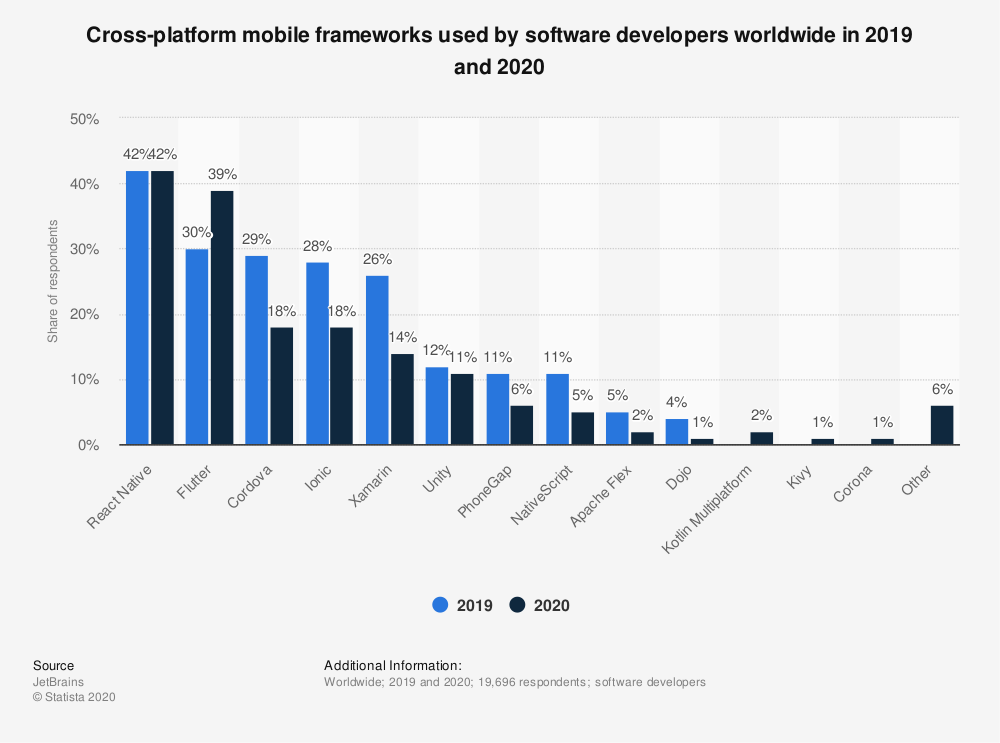
\includegraphics[scale=0.4]{images/crossplattform_popularity.png}
	\end{center}
	\caption{Beliebtheit nach Framework im Bereich der plattformübergreifenden mobilen Entwicklung \protect \footnotemark}
	\label{fig:crossplattform_popularity}
\end{figure}
\footnotetext{Quelle: \href{https://www.statista.com/statistics/869224/worldwide-software-developer-working-hours/}{www.statista.com}, zuletzt aufgerufen am 22.04.2021}

\subsubsection{React Native}
\label{react-native}
React Native ist ein open source Framework, welches von Facebook 2015 veröffentlicht wurde. 
Es basiert auf dem bekannten Web-Framework \href{https://reactjs.org/}{\textit{React}} (ebenfalls von Facebook) und bringt daher den deklarativen und Komponenten-basierten Stil mit sich. 
Die Programmiersprache ist aus diesem Hintergrund auch logischerweise JavaScript.
Das Framework an sich ist in verschiedenen Sprachen implementiert: JavaScript, Swift, Objective-C, C++ und Python.\\
\\
Allgemein bietet das Framework die Möglichkeit plattformübergreifende Apps für iOS, Android und für Windows zu schreiben. Hierbei wird der geschriebene Code in einer JavaScript Laufzeitumgebung ausgeführt (React Native selbst verwendet generell \href{https://trac.webkit.org/wiki/JavaScriptCore}{JSC (JavaScriptCore)}, seit neuestem kommt auch \href{https://hermesengine.dev/}{Hermes} zum Einsatz, jedoch sind auch andere bekannte Umgebungen denkbar - bspw. \href{https://v8.dev/}{V8} in Chrome) es lässt sich zu den Runtime-basierten Anwendungen in Kapitel \ref{runtime_based_apps} zuordnen. \cite{reactnative2021}\\
\paragraph{Architektur}
Grundlegend wurde React Native als Plattform-agnostisch designet. Entwickler schreiben also plattformunabhängigen JavaScript React Code, während das Framework den erstellten React Baum in Plattform-spezifischen Code umschreibt. Hierbei wurde 2013 (noch intern) die Web-Technologie React mit nativen Plattformen (nur interne) vereint, jedoch war dieses Design aufgrund eines einzigen Threads sehr langsam. Um dies zu verbessern basierte das Framework lange Zeit auf drei unterschiedlichen Threads, welche über eine Brücke verbunden sind.

\begin{figure}[h]
	\begin{center}
		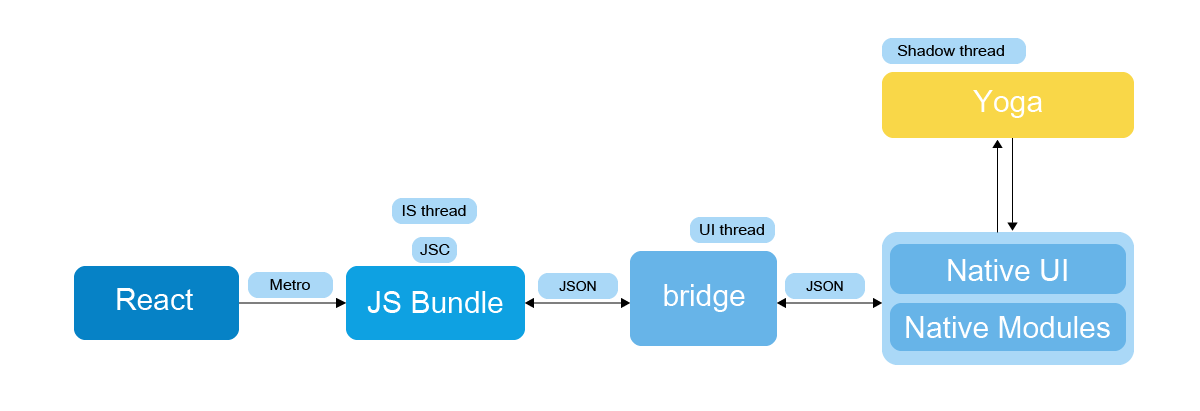
\includegraphics[scale=0.4]{images/reactnative_architecture_old.png}
	\end{center}
	\caption{Alte Architektur von React Native \protect \footnotemark}
	\label{fig:reactnative_architecture_old}
\end{figure}
\footnotetext{Quelle: \href{https://litslink.com/blog/new-react-native-architecture}{React Native Re-Architecture}, zuletzt aufgerufen am 15.04.2021}

\begin{itemize}
	\item \textit{JavaScript Thread}. Hier wird der gesamte JavaScript Code abgelegt und interpretiert. Alles wird über die JSC Engine ausgeführt.
	\item \textit{Native Thread}. Die Benutzeroberfläche und Kommunikation mit dem JavaScript Thread steht hier im Mittelpunkt. Der gesamte native Code wird hier ausgeführt. Die Benutzeroberfläche wird dann aktualisiert, sobald die eben ein Änderung vom JS Thread vermittelt wird.
	\item \textit{Shadow Thread}. Hier wird das gesamte Layout der Anwendung berechnet. Zugrunde liegt die Facebook-eigene layout engine \glqq Yoga\grqq .
\end{itemize}

Ein Hauptproblem dieses Ansatzes ist, dass die Brücke grundlegend eine asynchrone Warteschlange ist, da der JS Thread und der native Thread unabhängig voneinander arbeiten. Zusätzlich werden während der gesamten Datenübertragung die Daten im JSON Format serialisiert und deserialisiert .
Daher kann es zu Performance-Einbrüchen und somit zu schlechter Nutzererfahrung, durch bspw. Eingabeverzögerung, kommen.

\begin{figure}[h]
	\begin{center}
		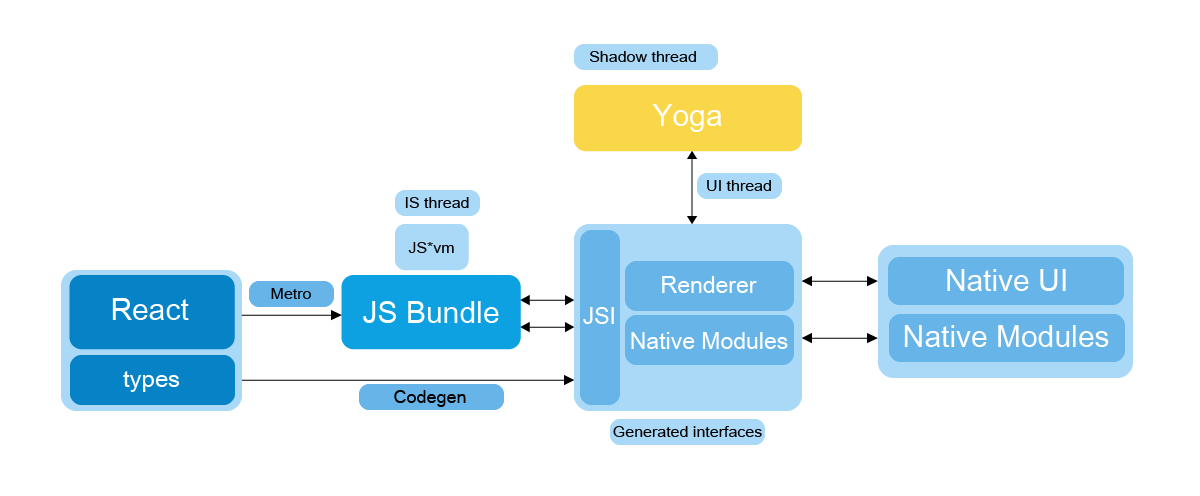
\includegraphics[scale=0.4]{images/reactnative_architecture.png}
	\end{center}
	\caption{Neue Architektur von React Native \protect \footnotemark}
	\label{fig:reactnative_architecture}
\end{figure}
\footnotetext{Quelle: \href{https://litslink.com/blog/new-react-native-architecture}{React Native Re-Architecture}, zuletzt aufgerufen am 15.04.2021}

Nach der Ankündigung 2018 veröffentlichte Facebook im Juli 2020 die neue Architektur. Mit ihr wurde der Bottleneck (die Brücke) ersetzt durch das JavaScript Interface. 
Es ermöglicht nicht nur die komplette Synchronisierung der beiden Threads, sondern auch die direkte Kommunikation untereinander - vor allem das Konzept von \glqq shared ownership\grqq ist hier tragend, weshalb auch keine Serialisierung mehr nötig ist.
Zudem  ist man nun nicht mehr an JSC gebunden, sondern kann auch jegliche hoch-performante JavaScript Engines als Laufzeitumgebung verwenden.
Native Module werden nun nur noch bei Bedarf geladen anstatt alle beim Start der App.\\
Weiter wurde veralteten Legacy-Code aus dem Kern von React Native entfernt und nicht-essenzielle Teile aus dem Kern ausgelagert. Dadurch zeigt sich die aktuelle Architektur von React Native in Abbildung \ref{fig:reactnative_architecture}.\footnote{Quelle: \href{https://medium.com/swlh/react-natives-re-architecture-in-2020-9bb82659792c}{React Native's re-architecture in 2020}}

\paragraph{JSX mit nativen Komponenten}
React (Native) verwendet als Programmiersprache JSX. Diese ist eine syntaktische Erweiterung von JavaScript (\textbf{J}ava\textbf{S}cript e\textbf{X}tention), welche zur fundamentalen Beschreibung der Nutzeroberfläche dient. JSX wird in normale JavaScript Objekte kompiliert, weshalb es nicht zwingend ist. \\
\begin{lstlisting}[caption=JSX Hello World Element]
	const element = <h1>Hello, world!</h1>;
\end{lstlisting}
Mithilfe dieser losen Kopplung von UI-Code und dazugehöriger Logik schlägt React eine optionale Lösung zur \textit{Separation of Concerns} vor. Anstelle dessen ist es auch möglich die Technologien in Markup- und Logik-Dateien aufzuteilen. \\
Außerdem könnte man argumentieren, das JSX einfach eine weitere Template-Sprache sei - ähnlich HTML oder XAML. Jedoch ist dies falsch, da (wie oben bereits erwähnt) JSX lediglich eine syntaktische Erweiterung von JavaScript ist, also man inmitten von JSX Objekten JavaScript schreiben kann.\\
Weiterhin ist interessant, dass JSX \href{https://owasp.org/www-community/attacks/xss/}{Cross Site Scripting} vorbeugt, indem der React DOM alle eingesetzte Werte zunächst als normalen String konvertiert. \cite{react2021}
\begin{lstlisting}[caption=Native Komponenten, label=lst:jsx_native_component]
	import React from 'react';
	import { Text } from 'react-native';
	
	const Cat = () => {
		return (
		// <Text> as native component
		<Text>Hello, I am your cat!</Text>
		);
	}
	
	export default Cat;
\end{lstlisting}
In dem Codebeispiel \ref{lst:jsx_native_component} wird ein Element \texttt{Cat} erzeugt, welches als Beschreibung dessen dient, was letztendlich auf dem Bildschirm angezeigt wird. 
In diesem einfachen Beispiel wird die native Komponente \texttt{<Text>...</Text>} verwendet. 
Native Komponenten sind in nativem Code (Kotlin oder Java für Android, bzw. Swift oder Objective-C für iOS) implementierte Komponenten und können in JavaScript Code aufgerufen werden. 
Diese werden dann während der Laufzeit für die jeweilige Plattform erstellt.\\
\\
React Native bringt die wichtigsten Komponenten mit sich, die \textbf{Core Components}. Zusätzlich erlaubt das Framework jedoch auch eigene Komponenten nativ zu implementieren, welche zum speziellen Anwendungsfall passen.\\

\paragraph{Komponenten}
Gleichzeitig erlaubt React Native aber auch wiederverwendbare Komponenten in JavaScript aus den Kernkomponenten zusammenstellen. 
Hierzu lassen sich einzelne Komponente jedoch nicht nur in einander verschachteln, um hier beispielsweise einen \texttt{Text} innerhalb einer \texttt{View}\footnote{Eine \texttt{View} ist die Basiskomponente einer Benutzeroberfläche. In einer \texttt{View} wiederum können wieder Views verschachtelt sein.} anzeigen zu lassen.
Zusätzlich ist es möglich sogenannte \glqq props\grqq also Eigenschaften (engl.: properties), ähnlich einer normalen Funktion mitzugeben. 
In diesem Beispiel sind das hier die Namen einzelner Katzen, welche als Text angezeigt werden. \cite{reactnative2021}\\

\begin{lstlisting}[caption=Eigene Komponenten, label=lst:reactnative_own_components]
import React from 'react';
import { Text, View } from 'react-native';

// configurable props
const Cat = (props) => {
	return (
	<View>
	<Text>Hello, I am {props.name}!</Text>
	</View>
	);
}

const Cafe = () => {
	return (
	<View>
	// reusable
	<Cat name="Maru" />
	<Cat name="Jellylorum" />
	<Cat name="Spot" />
	</View>
	);
}

export default Cafe;
\end{lstlisting}

Für eine interaktive Benutzeroberfläche fehlt jedoch noch das Kernprinzip eines deklarativen UI:\\

\paragraph{State}
wird verwendet um die Daten, welche sich mit der Zeit oder über Nutzerinteraktion ändern, auf der Oberfläche anzuzeigen. Dieses Konzept wird ebenfalls von dem zweiten Framework verwendet und ist in Abbildung \ref{fig:flutter_state} gut visualisiert.\\
\\
Um einer Funktion einen \textit{State} hinzuzufügen, ermöglicht React (und auch React Native) seit v16.8 dies durch Hooks. Hooks sind Funktionen, welche es Entwicklern ermöglicht sich in React Features einzuhaken. Bisher wurde dies über Klassen Komponenten ermöglicht, dadurch ist es jedoch komplizierter \textit{stateful logic} zwischen Komponenten wiederzuverwenden. Daher entkoppelt man diese Logik von den Komponenten und erlaubt unter anderem das separate Testen.


\begin{lstlisting}[caption=State mit \texttt{useState} Hook, label=lst:reactnative_state]
	import React, { useState } from "react";
	import { Button, Text, View } from "react-native";
	
	const Cat = (props) => {
		// make isHungry stateful
		const [isHungry, setIsHungry] = useState(true);
		
		return (
		<View>
		<Text>
		// show text dependent on isHungry state
		I am {props.name}, and I am {isHungry ? "hungry" : "full"}!
		</Text>
		<Button
		onPress={() => {
				setIsHungry(false);
		}}
		disabled={!isHungry}
		title={isHungry ? "Pour me some milk, please!" : "Thank you!"}
		/>
		</View>
		);
	}
	
	const Cafe = () => {
		return (
		<>
		<Cat name="Munkustrap" />
		<Cat name="Spot" />
		</>
		);
	}
	
	export default Cafe;
\end{lstlisting}

Im Beispiel \ref{lst:reactnative_state} wird in Zeile 6 der \texttt{useState} Hook verwendet. Die Funktion erzeugt eine State Variable mit dem Initialwert \texttt{true} und erstellt gleichzeitig eine Funktion zur Änderung des States (\texttt{setIsHungry}). Daraufhin wird abhängig ob die Katze hungrig ist, dies im Text angezeigt, der Knopf zum füttern (de-) aktiviert bzw. auch hier den Text verändert. \cite{reactnative2021}\\

\subsubsection{Flutter}
\label{flutter}
Flutter ist eine open-source SDK entwickelt von Google und ist geschrieben in C, C++ und Dart.
Flutter erlaubt es Anwendungen für Android, iOS, Web und Desktop basierend auf einem Code zu erstellen und ist zudem die primäre Methode für Google Fuchsia, Googles Betriebssystem.\footnote{Quelle: \url{https://fuchsia.dev/}}
Flutter verwendet \href{https://skia.org/}{Skia} als 2D Grafikbibliothek, welche auch von Chrome, Firefox und Android verwendet wird. Zudem basiert Flutter auf der Dart Plattform welche das Compilieren auf 32-bit und 64-bit ARM Prozessoren, auf Intel x64 Prozessoren und in JavaScript ermöglicht (siehe Abbildung \ref{fig:dart_plattform}). Daher ist Flutter eine, wie in Kap. \ref{compilierte_anwendungen} beschriebene kompilierte plattformübergreifende Anwendung

Während der Entwicklung werden Flutter Apps in einer Virtuellen Maschine (VM) gestartet, welche \textit{stateful hot reload} ermöglicht - bei Änderungen muss die App also nicht komplett neu kompiliert werden. Wird die App nun veröffentlicht, wird sie in die Maschinencode der beschriebenen Plattformen übersetzt.
\\

\begin{figure}[h]
	\begin{center}
		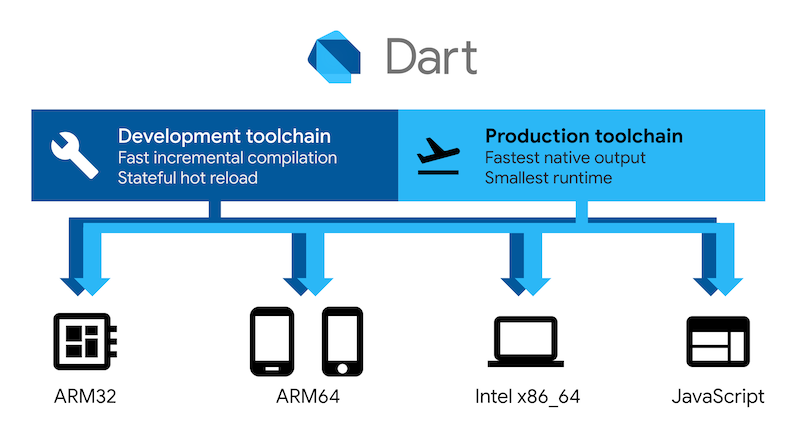
\includegraphics[scale=0.45]{images/dart-diagram.png}
	\end{center}
	\caption{Kompatibilität der Dart Plattform \protect \footnotemark}
	\label{fig:dart_plattform}
\end{figure}
\footnotetext{Quelle: \url{https://github.com/flutter/flutter}}

\paragraph{Architektur}
\begin{displayquote}
	Flutter is designed as an extensible, layered system. It exists as a series of independent libraries that each depend on the underlying layer. No layer has privileged access to the layer below, and every part of the framework level is designed to be optional and replaceable.\footnote{\url{https://flutter.dev/docs/resources/architectural-overview}}
\end{displayquote}

Grundlegend ist das Framework in drei Prozesseinheiten gegliedert. Diese bestehen wiederum jeweils aus, für sie charakteristischen APIs und Bibliotheken:

\begin{itemize}
	\item \textit{Flutter embedder}: Der Einstiegspunkt in die jeweilige Plattform. Er koordiniert Zugriffe auf Services des Betriebssystems; er ist also zuständig für bspw. die Kommunikation mit dem Input Method Editor (IME) und den Lifecycle Events der App. Daher ist der Embedder in der, von der Plattform unterstützten Programmiersprache geschrieben: derzeit wird Java und C++ für Android, Objective-C/Objective-C++ für iOS und macOS, und C++ für Windows und Linux verwendet.
	\item \textit{Flutter Engine}: Der Kern von Flutter, geschrieben hauptsächlich in C und C++, ist die \textit{low-level} Implementierung der Flutter Kern Programmierschnittstelle (API). Daher ist sie zuständig für das graphische Darstellen (Rasterisierung) des Codes sobald ein neuer \textit{Frame} angezeigt werden muss. Im Flutter Framework wird die \textit{Engine} als dart:ui Bibliothek offengelegt - der zugrundeliegende C++ Code wird in Dart Klassen eingefügt. 
	\item \textit{Flutter Framework}: Das Framework, mit welchem der Entwickler schlussendlich meistens arbeiten wird. Es ist in Dart geschrieben und bietet sogenannte \textit{Layer} für Animationen, Layout und Widgets. Widgets werden von Flutter als Einheit der Komposition von Benutzeroberflächen verwendet und sind als einzelne Bausteine zu verstehen, welche zusammengefügt ein Objekt oder sogar einen kompletten Bildschirm ergeben.
\end{itemize}

Bei der Entwicklung mit Flutter wird ein Baum von Widgets erzeugt, welcher als Bauplan der Applikation angesehen werden kann. Nach diesem Plan wird mithilfe von States der einzelnen Widgets schlussendlich das User Interface (UI) gerendert.\cite{flutter2021}

\begin{figure}[tbt]
	\begin{center}
		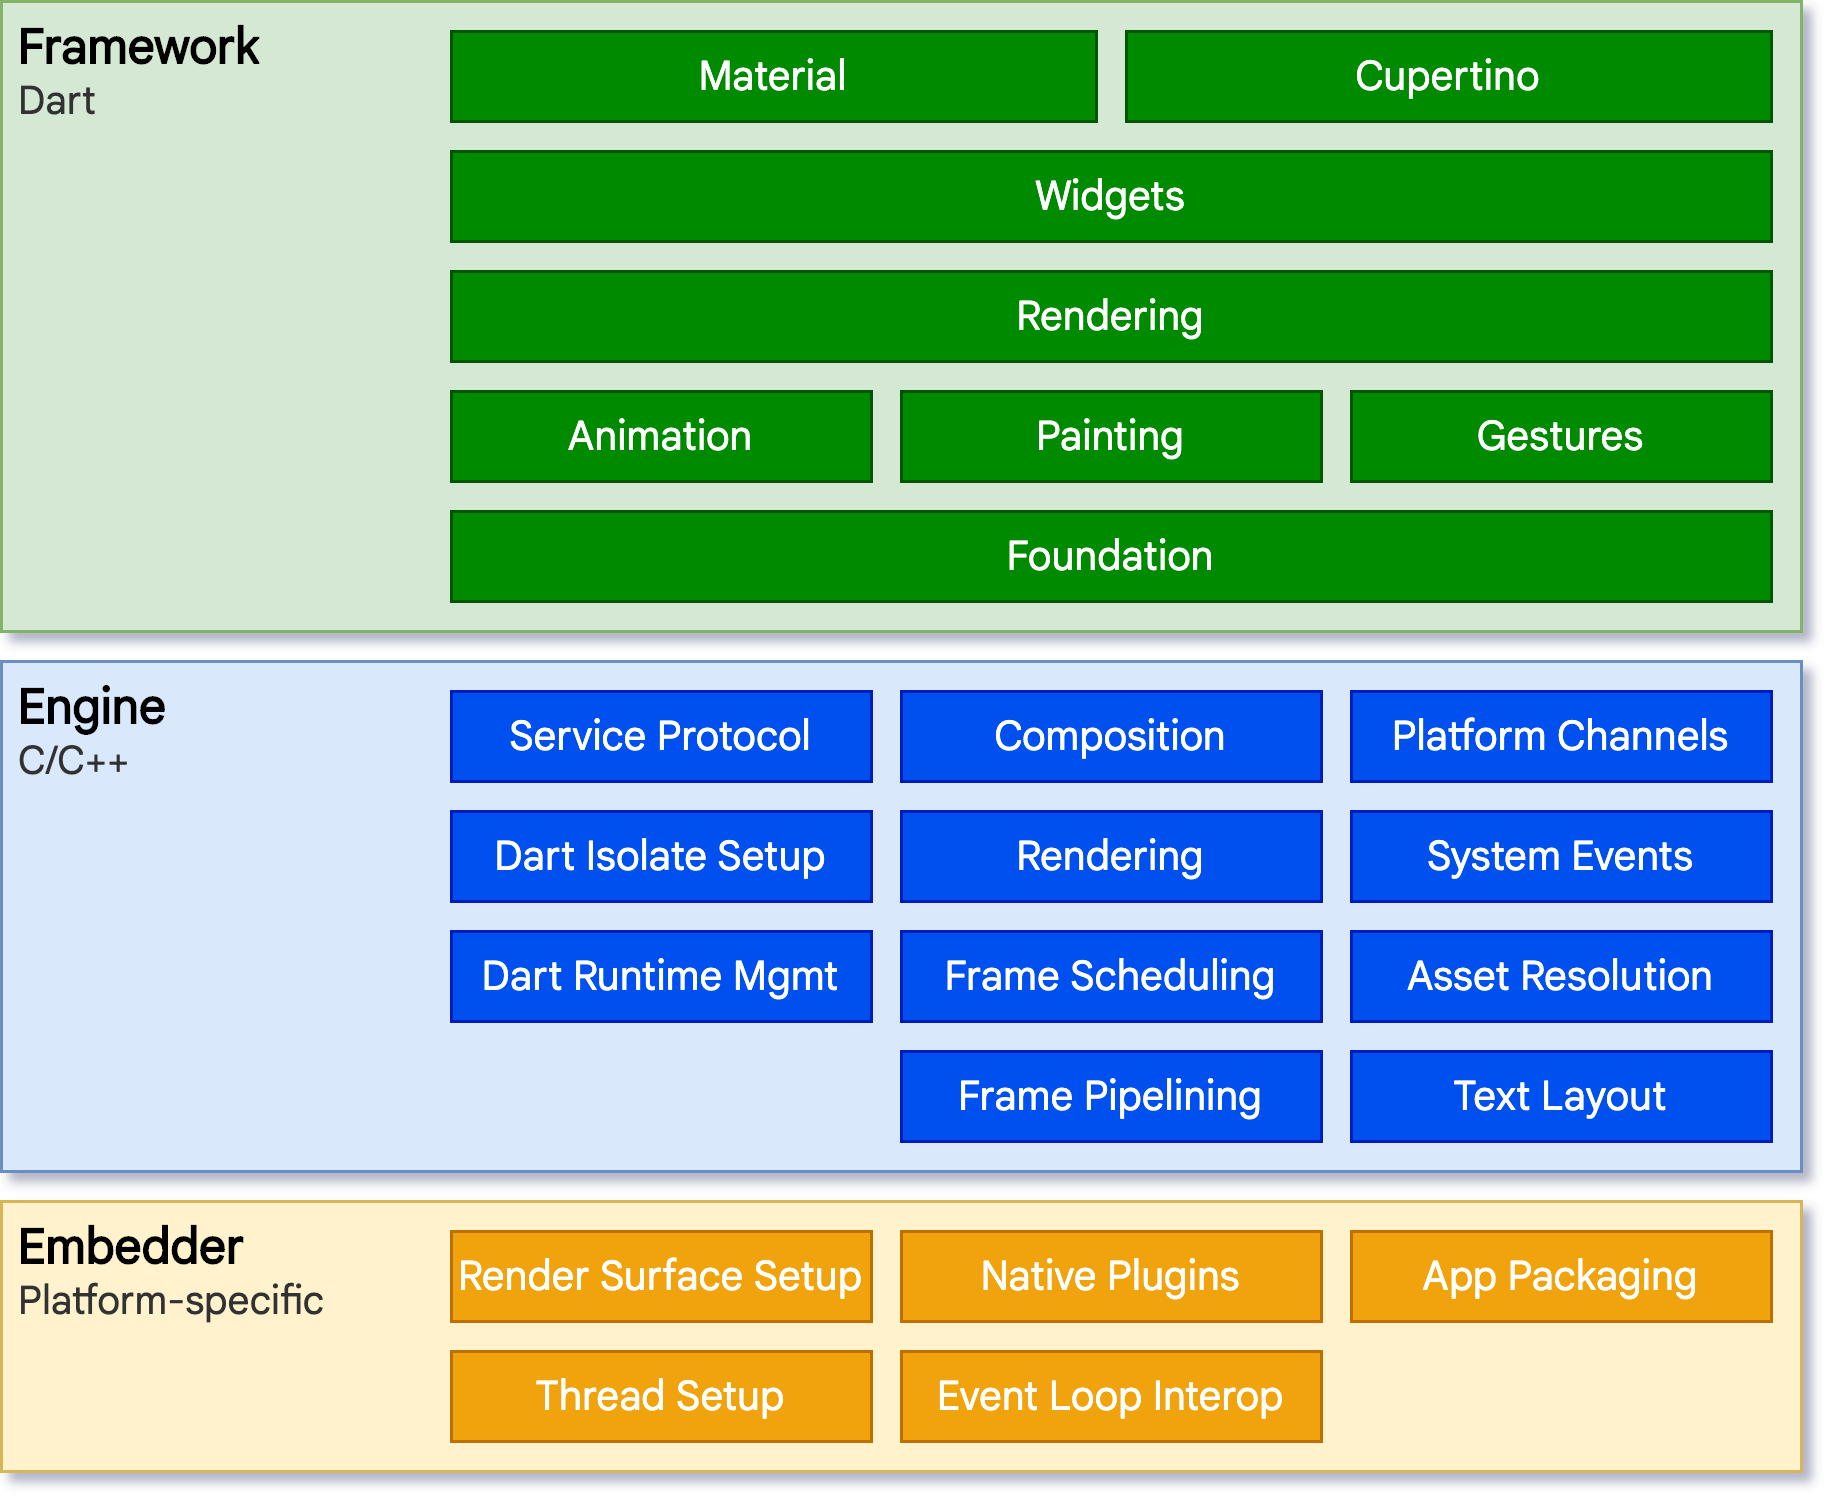
\includegraphics[scale=0.25]{images/flutter_architektur.png}
	\end{center}
	\caption{Bibliotheken und Ebenen der Flutter Plattform \protect \footnotemark}
	\label{fig:flutter_plattform}
\end{figure}
\footnotetext{Quelle: \url{https://github.com/flutter/flutter}}

\paragraph{Dart}
Während der Entwicklung von Flutter standen sicherlich mehrere Sprachen zur Auswahl: \\Wie in Kapitel \ref{plattformuebergreifende_anwendungen} gelernt, gibt es viele unterschiedliche Ansätze mit beispielsweise webbasierten Sprachen wie JavaScript, mit nativen Sprachen wie Java oder Swift, oder auch mit anderen objektorientierten Sprachen wie C\#. Wieso wurde also genau Dart als Programmiersprache und Runtime ausgewählt?\\
\\
Dart allgemein ist C ähnlich, also für viele Entwickler leicht(er) leserlich. Es ist eine objekt-orientierte Sprache und besitzt einen Garbage Collector.\\
Dart ist designet als eine Client-fokussierte Sprache, welche gleichermaßen Entwicklung (sub-second stateful hot reload) und Produktion in allen möglichen Zielplattformen (Web, Mobile und Desktop) priorisiert. Dadurch erhält man mit dieser Sprache eine Effizienz optimierte Entwicklungsphase, sowie ebenfalls die Möglichkeit eine Code-Basis in unterschiedliche Plattformen zu kompilieren (siehe Abbildung \ref{fig:dart_plattform}).\\
Es bietet zudem auch \textit{sound-null-safety} - Werte können also nicht null sein, außer man legt dies fest. Damit kann es null Exceptions während der Laufzeit durch statische Code Analyse vorbeugen.

\paragraph{Widgets}
Wie bereits beschrieben sind Widgets wiederverwendbare Kompositionsbausteine, mit welchen Benutzeroberflächen in Flutter zusammengebaut werden. Jedes einzelne ist ein \textit{immutable declaration} eines Teils der Benutzeroberflächen - also ein konstanter Bestandteil.\\
\\
Flutter arbeitet mit der Devise: 
\begin{displayquote}
	\textbf{\textit{Everything is a widget.}}
\end{displayquote}
Auf diesem Satz baut die Einfachheit von Flutter auf. Jedes Objekt, jede Animation, jede Reihe, einfach alles ist ein Widget. Somit baut man eine App von der Wurzel aus auf und beschreibt die einzelnen Abzweigungen exakt.
Die Anordnung von Widgets ist daher hierarchisch aufgebaut. 
Ein Widget wir also immer in einem Elternteil verschachtelt sein und erhält bei seiner Erstellung den \textit{build context} übergeben. Das \glqq äußerste\grqq \space Widget, also die Wurzel, enthält somit die gesamte App. Typischerweise ist das ein \textit{MaterialApp} oder \textit{CupertinoApp} Widget.\\
\\ 
OEM Widgets, also Widgets von und für eine spezifische Plattform werden von Flutter gemieden. Hierfür erzeugt Flutter eigene Widgets mithilfe der oben genannten, eigener Rendering Plattform. Da diese Widgets jedoch komplett individualisierbar sind, bietet man somit native Möglichkeiten für jegliche Stile. Es gibt auch Pakete, welche Plattform-ähnliche Widgets zur Verfügung stellen.

\begin{figure}[tbt]
	\begin{center}
		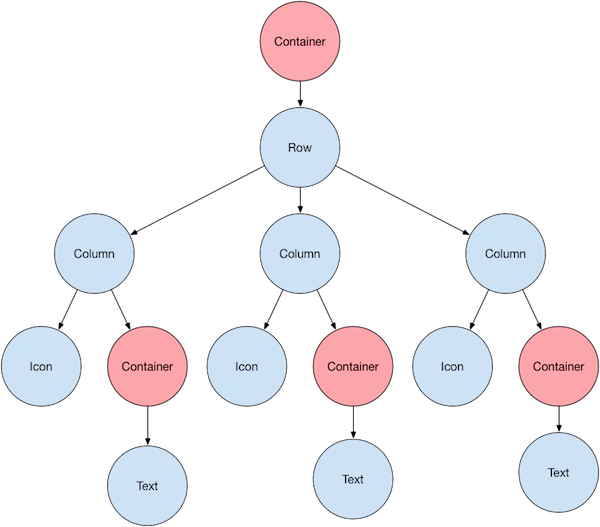
\includegraphics[scale=0.5]{images/flutter_widget_tree.png}
	\end{center}
	\caption{Widget Baum einer beispielhaften Anwendung \protect \footnotemark}
	\label{fig:flutter_widget_tree}
\end{figure}
\footnotetext{Quelle: \url{https://flutter.dev/docs/development/ui/layout}}
	

\paragraph{States}
Flutter ist deklarativ - das bedeutet, die Benutzeroberfläche wird anhand von dem aktuellen \textit{State} der App erzeugt. Im Gegensatz dazu muss der Entwickler beim imperativen Stil die Übergänge der einzelnen \textit{States}. Hier wird dies durch das Framework gelöst.
	
\begin{figure}[H]
	\begin{center}
		
\includegraphics[scale=0.4]{images/flutter_state.png}
	\end{center}
	\caption{Deklarative Benutzeroberfläche \protect \footnotemark}
	\label{fig:flutter_state}
\end{figure}
\footnotetext{Quelle: \url{https://flutter.dev/docs/development/data-and-backend/state-mgmt/declarative}}








\subsection{Language}
Hier steht mein Language Text.

\subsection{IDE}
Hier steht mein IDE Text.

\subsection{Database}
Hier steht mein Database Text.

\subsection{Firebase}
Firebase ist eine Backend-as-a-Service (BaaS) Plattform von Google für mobile oder Web-Anwendungen. 
Sie soll es dem Entwickler ermöglichen, einfacher und effizienter Funktionen auf verschiedenen Plattformen bereitzustellen stellt Tools und Infrastruktur zur Verfügung.
Mit dem Firebase SDK bietet die Plattform API Schnittstellen zu den jeweiligen Tools, welche direkt in die Anwendung integriert werden können, ohne dass serverseitiger Code dafür notwendig ist.
Die Firebase Inc. wurde 2011 von James Tamplin und Andrew Lee gegründet und letztendlich 2014 von Google übernommen.\footnote{\href{https://firebase.googleblog.com/2014/10/firebase-is-joining-google.html}{firebase.googleblog.com}, zuletzt aufgerufen am 03.05.2021}
Teile der SDK stehen seit der Google I/O 2017 unter der Apache 2.0 Lizenz, sind somit also Open-Source.\footnote{\href{https://opensource.googleblog.com/2017/05/open-sourcing-firebase-sdks.html}{opensource.googleblog.com}, zuletzt aufgerufen am 03.05.2021}\\
\\
Es existieren zwei Kostenmodelle für die Nutzung von Firebase: Ein kostenloses Modell \glqq Spark Plan\grqq und ein pay-as-you-go \glqq Blaze Plan\grqq . Das kostenlosen Modell beinhaltet die wichtigsten Tools, viele dieser Tools sind jedoch begrenzt durch beispielsweise Bandbreite oder Speicherplatz.
Der Pay-as-you-go Plan ist eine Erweiterung des kostenlosen Plans. 
Er bietet daher das Nutzen von Tools bis zu einem gewissen Limit kostenfrei an; darüber hinaus kostet es jedoch dann pro Nutzung.\\
\\
Ein Firebase Projekt ist die oberste Ebene in Firebase. 
Ein Projekt ist letztendlich ein \textit{Google Cloud Projekt}, welches mit speziellen Konfigurationsmöglichkeiten und Services ausgestattet ist. 
Es beinhaltet die Verknüpfung zu den einzelnen Anwendungen (also bspw. Android-, iOS- oder Webanwendung). Nun können variabel Tools, sog. Firebase products hinzugefügt werden. Diese Produkte lassen sich grundlegend in drei Kategorien einteilen. Die hier relevantesten werden im Folgenden besprochen.\cite{firebase2021}

\subsubsection{Firebase Authentifizierung}
Die Authentifizierung gehört zu den \glqq Build\grqq Produkten und bietet eine Token-basierte Nutzerauthentifizierung. 
Hierbei kann zwischen verschiedenen Anmeldeoptionen gewählt werden: klassisch mit E-Mail und Passwort, mit OAuth2.0 Integration für Social Media (Google, Facebook, Twitter, Github, ...) oder per Telefonnummer.
Jeder Nutzer erhält eine einzigartige ID und ein zugehöriges Nutzerobjekt in einer NoSQL Datenbank. Grundlegende Werte wie E-Mail Adresse oder Name können hier abgespeichert werden; zusätzliche Informationen müssen über einen weiteren Datenbank Service abgespeichert werden.
Für die Verwaltung eines Accounts bietet dieses Tool auch eingebaute E-Mail Aktionen an - bspw. Passwort zurücksetzen oder E-Mail Adresse bestätigen.\\
\\
Ein Firebase Nutzer Objekt repräsentiert den Account eines Nutzers, welcher sich von einer Anwendung aus beim zentralen Firebase Projekt angemeldet hat.
Die Instanz eines Firebase Nutzers ist somit unabhängig von der Authentifizierungsinstanz der Anwendung, also kann eine Anwendung mehrere Nutzer anmelden, jedoch kann sich auch ein Nutzer auf mehreren Anwendungen anmelden.
Ist ein Nutzer authentifiziert, erhält die Anwendung eine Referenz des Nutzers, welche so lange existiert, bis er wieder abgemeldet ist.\cite{firebase2021}

\subsubsection{Cloud Firestore}
\label{sec:firestore}
Als Datenbank Lösung bietet Firebase zwei unterschiedliche Produkte an: Cloud Firestore und Realtime Database.
Firestore ist hier neuer, jedoch ersetzt es Realtime Database nicht. \\
Cloud Firestore ist eine flexible und auf Skalierung ausgesetzte NoSQL Cloud Datenbank, welche unter anderem die Echtzeitsynchronisierung der Daten zwischen Anwendung und Server ermöglicht.
Zusätzlich zu REST und RPC APIs in iOS, Android und web SDKs ist Firestore auch in nativen Node.js, Java, Python und Go SDKs verfügbar.\\
\\

\begin{wrapfigure}{R}{0.4\textwidth}
	\begin{center}
		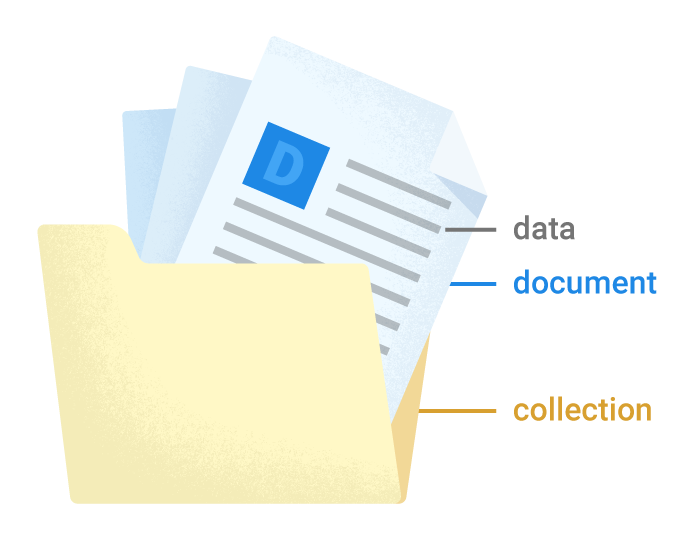
\includegraphics[width=0.35\textwidth]{images/firestore_datastucture.png}
	\end{center}
	\caption{Datenmodell in Firebase \protect \footnotemark}
	\label{fig:firestore_data_structure}
\end{wrapfigure}
\footnotetext{Quelle: \cite{firebase2021}}

Das Datenmodell ist hierarchisch aufgebaut, wobei Daten in Dokumenten (documents) und Dokumente in Sammlungen (collections) gespeichert sind. 
Mithilfe von Sammlungen werden die Daten voneinander abgetrennt und hierüber können Abfragen erstellt werden.
Grundlegende Datentypen sind String, Integer und Boolean, jedoch können auch komplexe Datentypen wie Maps, Arrays oder Geopoints. Unter-Sammlungen und darin verstaute Dokumente sind ebenfalls möglich.\\
\\
Abfragen werden auf Dokumentenebene erstellt, damit nicht eine gesamte Sammlung aufgerufen werden muss.
Dies kann über direkte Sortierung, Filter und/oder Limitierung bzw. genaue Auswahl eines Dokumentes bewerkstelligt werden.
Bei einer Abfrage erhält man einen \textit{Data Snapshot}, wodurch über Änderungen in Echtzeit informiert und diese angezeigt werden können.
Damit es jedoch zu keinen fehlerhaften Daten führt, gelten hier atomare Eigenschaften für Transaktionen.
Eine Transaktion ist eine Folge von Datenbankanweisungen, welche entweder alle gemeinsam oder gar nicht ausgeführt werden. 
Eine Transaktion ist nur dann erfolgreich, wenn alle Anweisungen auf eine Datenbank vollständig geschlossen sind. 
Ist dies nicht der Fall, werden alle Anweisungen bis zum Stand vor der Transaktion rückgängig gemacht. Das nennt man Rollback.\\
\\
Die Sicherheit der Daten stellt Cloud Firestore für Mobil- und Webclient-Bibliotheken über die Firestore-Sicherheitsregeln her. Diese bieten sowohl Zugriffsverwaltung und -authentifizierung, jedoch könne auch Daten hiermit für die Konsistenz der Datenbank validiert werden. 
\medskip
\begin{lstlisting}[caption=Beschränkung des Zugriffs auf Dokumente der Sammlung \texttt{cities}, label=lst:firestorerules_basic]
	service cloud.firestore {
		match /databases/{database}/documents {
			match /cities/{city} {
				allow read, write: if request.auth != null;
			}
		}
	}
\end{lstlisting}
\medskip
Im Beispiel \ref{lst:firestorerules_basic} wird der Lese- und Schreibzugriff auf ein Dokument der Sammlung \texttt{cities} beschränkt. 
Nur falls der anfragende Nutzer eine valide Authentifizierung besitzt, erhält er Zugriff auf das angefragte Dokument. 
Diese simple Darstellung ist jedoch für den wirklichen Produktionseinsatz mit Vorsicht zu nutzen. 
Oftmals müssen \texttt{read} und \texttt{write} in detailliertere Vorgänge aufgeteilt werden. Ein \texttt{read} wird spezialisiert in \texttt{get} und \texttt{list}, wobei ein \texttt{write} in \texttt{create}, \texttt{update} und \texttt{delete} unterteilt werden kann.
Ein \texttt{list} ermöglicht es hierbei auf Sammlungen, also die einzelnen Dokumenten IDs lesend zuzugreifen, jedoch nicht auf die Daten einzelner Dokumente. Hierfür wird dann ein \texttt{get} benötigt. 
Mittels \texttt{create} erhält man Schreibzugriff auf nicht existierende Dokumente, durch \texttt{update} auf bereits vorhandene und Löschrechte ganzer Dokumente erhält man über den \texttt{delete} Operator.\\
\\
Sicherheitsregeln werden gleich dem Datenmodell hierarchisch aufgebaut und ermöglichen differenzierte Zugriffsbeschränkungen auf jeder Ebene.
In Codebeispiel \ref{lst:firestorerules_hierarchy} beinhaltet jedes Dokument (Stadt) der Sammlung \texttt{cities} eine Unter-Sammlung \texttt{landmarks}. Nun lässt sich der Zugriff auf beide separat regeln.
Bei der Sammlung \texttt{villages} hingegen wurde der rekursive Platzhalter verwendet. Hiermit sind Zugriffsregeln auf allen tieferen Ebenen gleich.
Beim Verschachteln von \texttt{match} ist der innere Pfad immer relativ zum äußeren.

Wichtig zu wissen ist hierzu noch, dass falls mehrere \texttt{allow} Ausdrücke auf eine Anfrage zutreffen, wird der Zugriff erlaubt sobald \textbf{eine} Bedingung wahr, also erfüllt ist.

\medskip
\begin{lstlisting}[caption=Hierarchische Zugriffsbeschränkung, label=lst:firestorerules_hierarchy]
	service cloud.firestore {
		match /databases/{database}/documents {
			match /cities/{city} {
				allow read, write: if <condition>;
				
				// Explicitly define rules for the 'landmarks' subcollection
				match /landmarks/{landmark} {
					allow read, write: if <condition>;
				}
			}
			match /villages/{document=**} {
				allow read, write: if <condition>;
			}
		}
	}
\end{lstlisting}
\medskip

Wie bereits oben besprochen können diese Regeln auch zur Validierung von Daten genutzt werden, damit die atomare Eigenschaft von Transaktionen bestehen bleibt.
Hierzu kann die \texttt{getAfter()} Funktion genutzt werden. 
Mit dieser kann man auf Zustand eines Dokumentes zugreifen und diesen validieren, nachdem einer Folge von Anweisungen ausgeführt, jedoch diese noch nicht auf der Firestore Datenbank abgeschlossen wurde.
Im Beispiel \ref{lst:firestorerules_validation} existieren zwei Sammlungen: \texttt{cities} und \texttt{countries}. 
Jedes \texttt{country} Dokument beinhaltet das Feld \texttt{last\_updated} um zu wissen, welche Stadt innerhalb eines Landes zuletzt aktualisiert wurde.
Hierzu wird in den Sicherheitsregeln nach jedem Schreibzugriff auf ein \texttt{city} Dokument gleichzeitig auch das Feld des zugehörigen Landes aktualisiert.\cite{firebase2021}
\medskip
\begin{lstlisting}[caption=Datenvalidierung für atomare Operationen, label=lst:firestorerules_validation]
	service cloud.firestore {
		match /databases/{database}/documents {
			// If you update a city doc, you must also
			// update the related country's last_updated field.
			match /cities/{city} {
				allow write: if request.auth != null &&
				getAfter(
				/databases/$(database)/documents/countries/$(request.resource.data.country)
				).data.last_updated == request.time;
			}
			
			match /countries/{country} {
				allow write: if request.auth != null;
			}
		}
	}
\end{lstlisting}
\medskip

\subsubsection{Cloud Storage}
Um Filme, Videos oder andere Nutzer-generierte Inhalte abspeichern zu können, bietet Firebase Cloud Storage an. 
Durch das Firebase SDK für Cloud Storage können Dateien direkt von Client-Anwendungen hoch- bzw. heruntergeladen werden.
Aufgrund von möglicher schlechter Verbindung kann mithilfe von robusten Operationen der Prozess des Hoch- bzw. Herunterladens bei besserer Verbindung an der Stelle weiter geladen werden, an welcher dieser unterbrochen wurde.
Ähnlich wie bei Cloud Firestore in Kapitel \ref{sec:firestore} bestimmen auch hier Sicherheitsregeln den Zugriff auf bestimmte Dokumente.\\
Zusätzlich hierzu sind weitere Metadaten verfügbar: \texttt{contentType} und \texttt{size}. 
Mit ihnen lassen sich die Dateien beispielsweise validieren.
Im Code \ref{lst:storagerules_validation} können Dateien nur hochgeladen werden, falls sie eine Größe kleiner 5 MB besitzen.
\medskip
\begin{lstlisting}[caption=Validierung nach Dateigröße, label=lst:storagerules_validation]
	service firebase.storage {
		match /b/{bucket}/o {
			match /images/{imageId} {
				allow write: if request.resource.size < 5 * 1024 * 1024
				&& request.resource.contentType.matches('image/.*');
			}
		}
		
\end{lstlisting}
\medskip
Außerdem lassen sich durch Cloud Functions aus dem nächsten Kapitel Prozesse automatisieren. Beispielsweise lässt sich beim Upload eines Bildes direkt ein individuelles Thumbnail erstellen lassen.\cite{firebase2021}
\subsubsection{Cloud Functions}
\label{sec:cloudfunctions}
Da Firebase - bis auf vereinfachte Sicherheitsregeln - eigentlich keinen Backend Code benötigt, jedoch manche Features eben genau diesen brauchen, um beispielsweise Benachrichtigungen an Nutzer zu senden oder Bilder zu komprimieren, existieren Cloud Functions.\\
Diese ermöglichen es, als Antwort auf ein Event automatisch oder durch HTTPS Anfrage manuell Backend Code auszuführen.
Der gesamte Code ist hierbei in der Google Cloud gespeichert und wird in einer verwalteten Umgebung ausgeführt.
Als Programmiersprache kann sowohl JavaScript als auch Typescript verwendet werden.\\
\\
\glqq Google Cloud Functions ist die serverlose Computerlösung von Google zum erStellen ereignisgesteuerter Anwendungen.\grqq \cite{firebase2021} 
Es kann sowohl auf der Google Cloud Platform (GCP) also auch für Firebase genutzt werden. 
Es ist bei beiden ein Verbindungsglied zwischen Logik und entsprechenden Diensten, welche dadurch mit serverseitigen Code erweitert und kombiniert werden.
\begin{figure}[htb]
	\begin{center}
		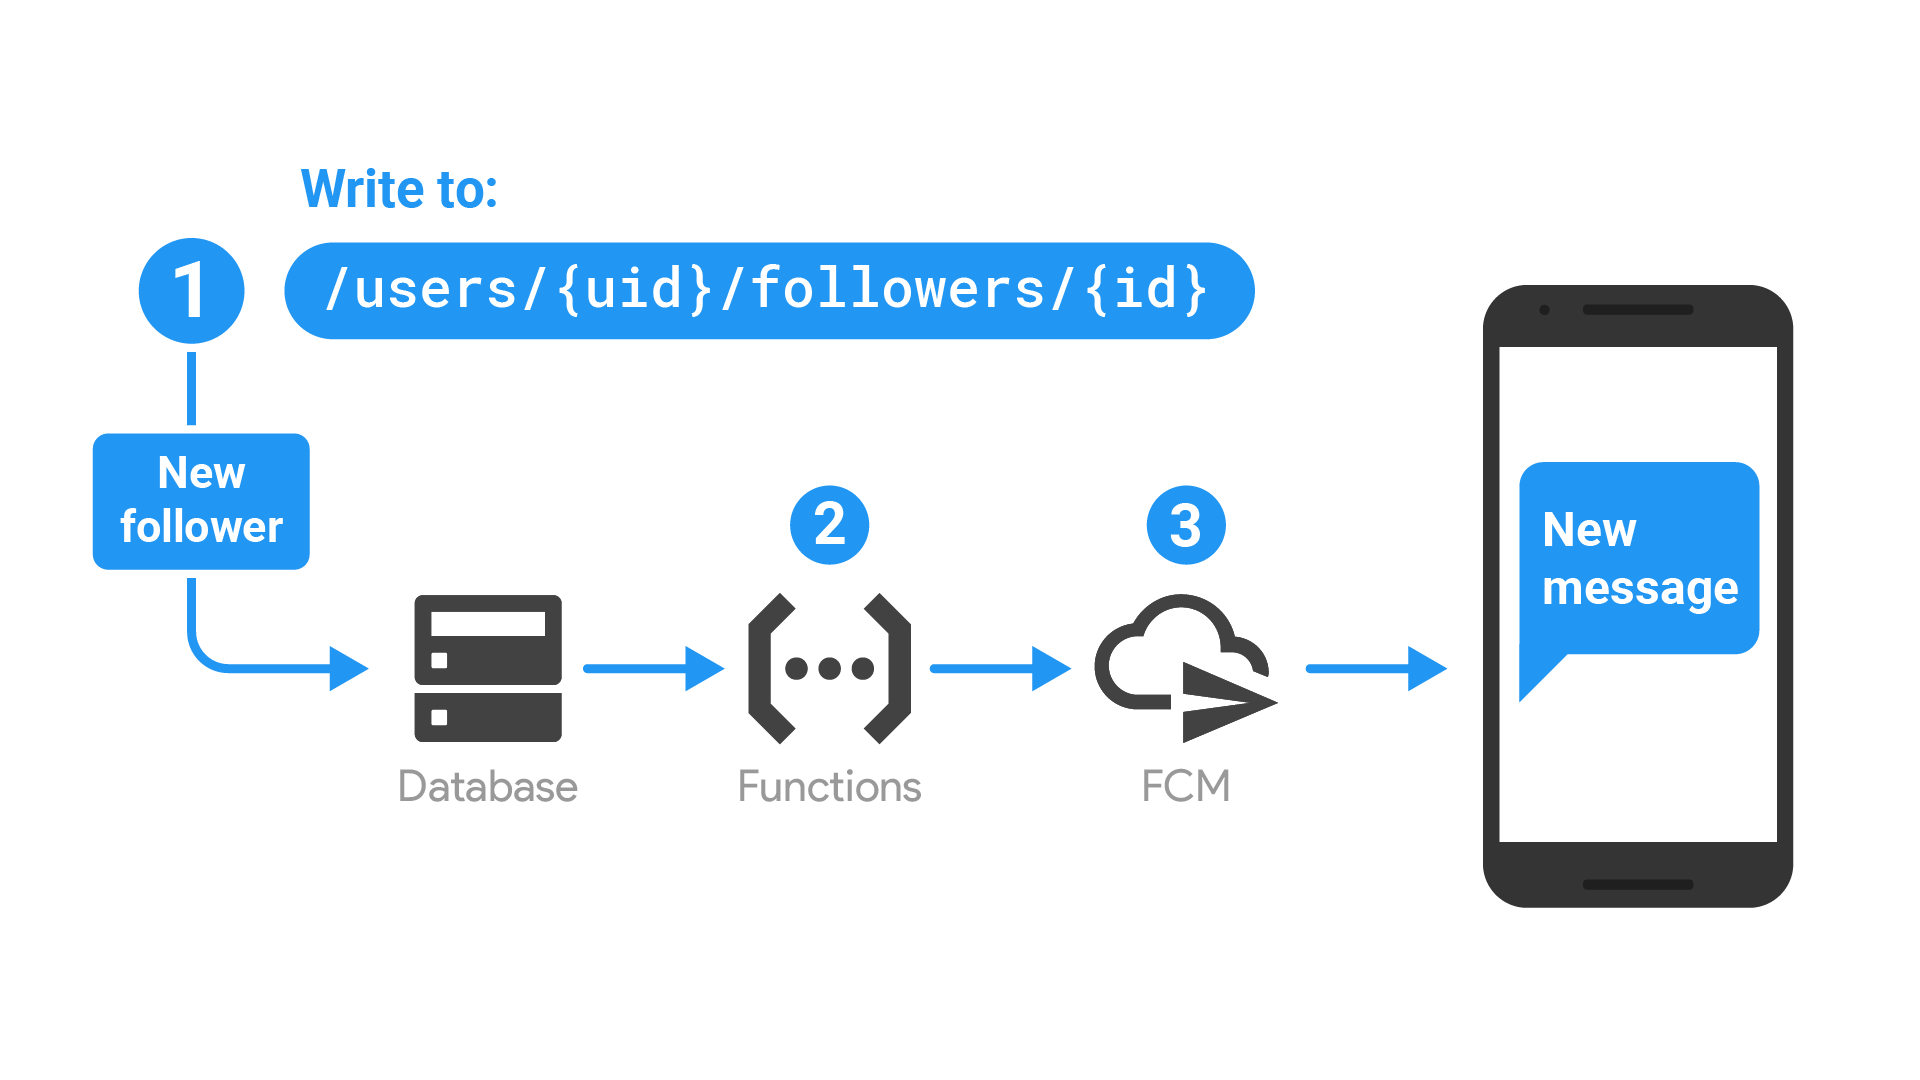
\includegraphics[scale=0.2]{images/firebase_functions_notify.png}
	\end{center}
	\caption{Cloud Functions Anwendungsfall Benachrichtigung}
	\label{fig:functions_notifications}
\end{figure}
In Abbildung \ref{fig:functions_notifications} ist ein typischer Anwendungsfall beschrieben. 
Ein Event auf der Datenbank wird ausgelöst, hier ein neuer Nutzer folgt einem weiteren Nutzer.
Es wird also ein Dokument in der Unter-Sammlung \texttt{followers} erzeugt. Diese Unter-Sammlung befindet sich innerhalb des Dokumentes \texttt{uid} der Sammlung \texttt{users}.
Im zweiten Schritt erstellt die Funktion eine Nachricht, welche über Firebase Cloud Messaging (FCM) versendet werden soll.
Über abgespeicherte Tokens sendet FCM die Benachrichtigung an das Gerät des Nuters \texttt{uid}.\cite{firebase2021}
\subsubsection{Cloud Messaging}
Firebase Cloud Messaging ist eine plattformübergreifende Messaging-Lösung zum zuverlässigen Versenden von Nachrichten an Nutzergeräte.
In Abbildung \ref{fig:cloudmessaging_architecture} ist die Architektur dieses Tools dargestellt.
Hierbei wird es grundlegend in das Erstellen, Transportieren und Empfangen der Nachrichten unterteilt.\cite{firebase2021}\\
\begin{itemize}
	\item \textbf{Erstellen} Die zu versendenden Nachrichten können, wie in Kapitel \ref{sec:cloudfunctions} beschrieben, manuell oder automatisiert erzeugt werden. 
	Bei der Automatisierung ist wichtig, dass die Nachrichten in einer vertrauenswürdigen Serverumgebung erstellt werden, damit alle Nachrichtentypen unterstützt werden (Schritt 1). 
	Das FCM Backend akzeptiert dann in Schritt 2 Nachrichtenanfragen, ordnet die Nachrichten verschiedenen Themen zu und erzeugt unter anderem Metadaten für Nachrichten, wie bspw. die Nachricht ID. 
	\item \textbf{Transportieren} Die Nachrichten werden hierbei an die entsprechenden Geräte weitergeleitet.
	Da verschiedene Geräte auf unterschiedlichen Plattformen basieren, muss die Transportschicht auf Plattformebene arbeiten.
	Hierfür werden folgende Ebenen genutzt:
	\begin{itemize}
		\item Android Transport Layer (ATL) für Android-Geräte mit Google Play-Diensten
		\item Apple Push Notification Service (APNs) für iOS-Geräte
		\item Web-Push-Protokoll für Web-Apps
	\end{itemize}
	\item \textbf{Empfangen} Das FCM SDK behandelt die Benachrichtigung oder Nachricht. Dies ist abhängig vom Vorder-/ Hintergrundstatus der Anwendung und der jeweiligen Anwendungslogik.
\end{itemize}


\begin{figure}[htb]
	\begin{center}
		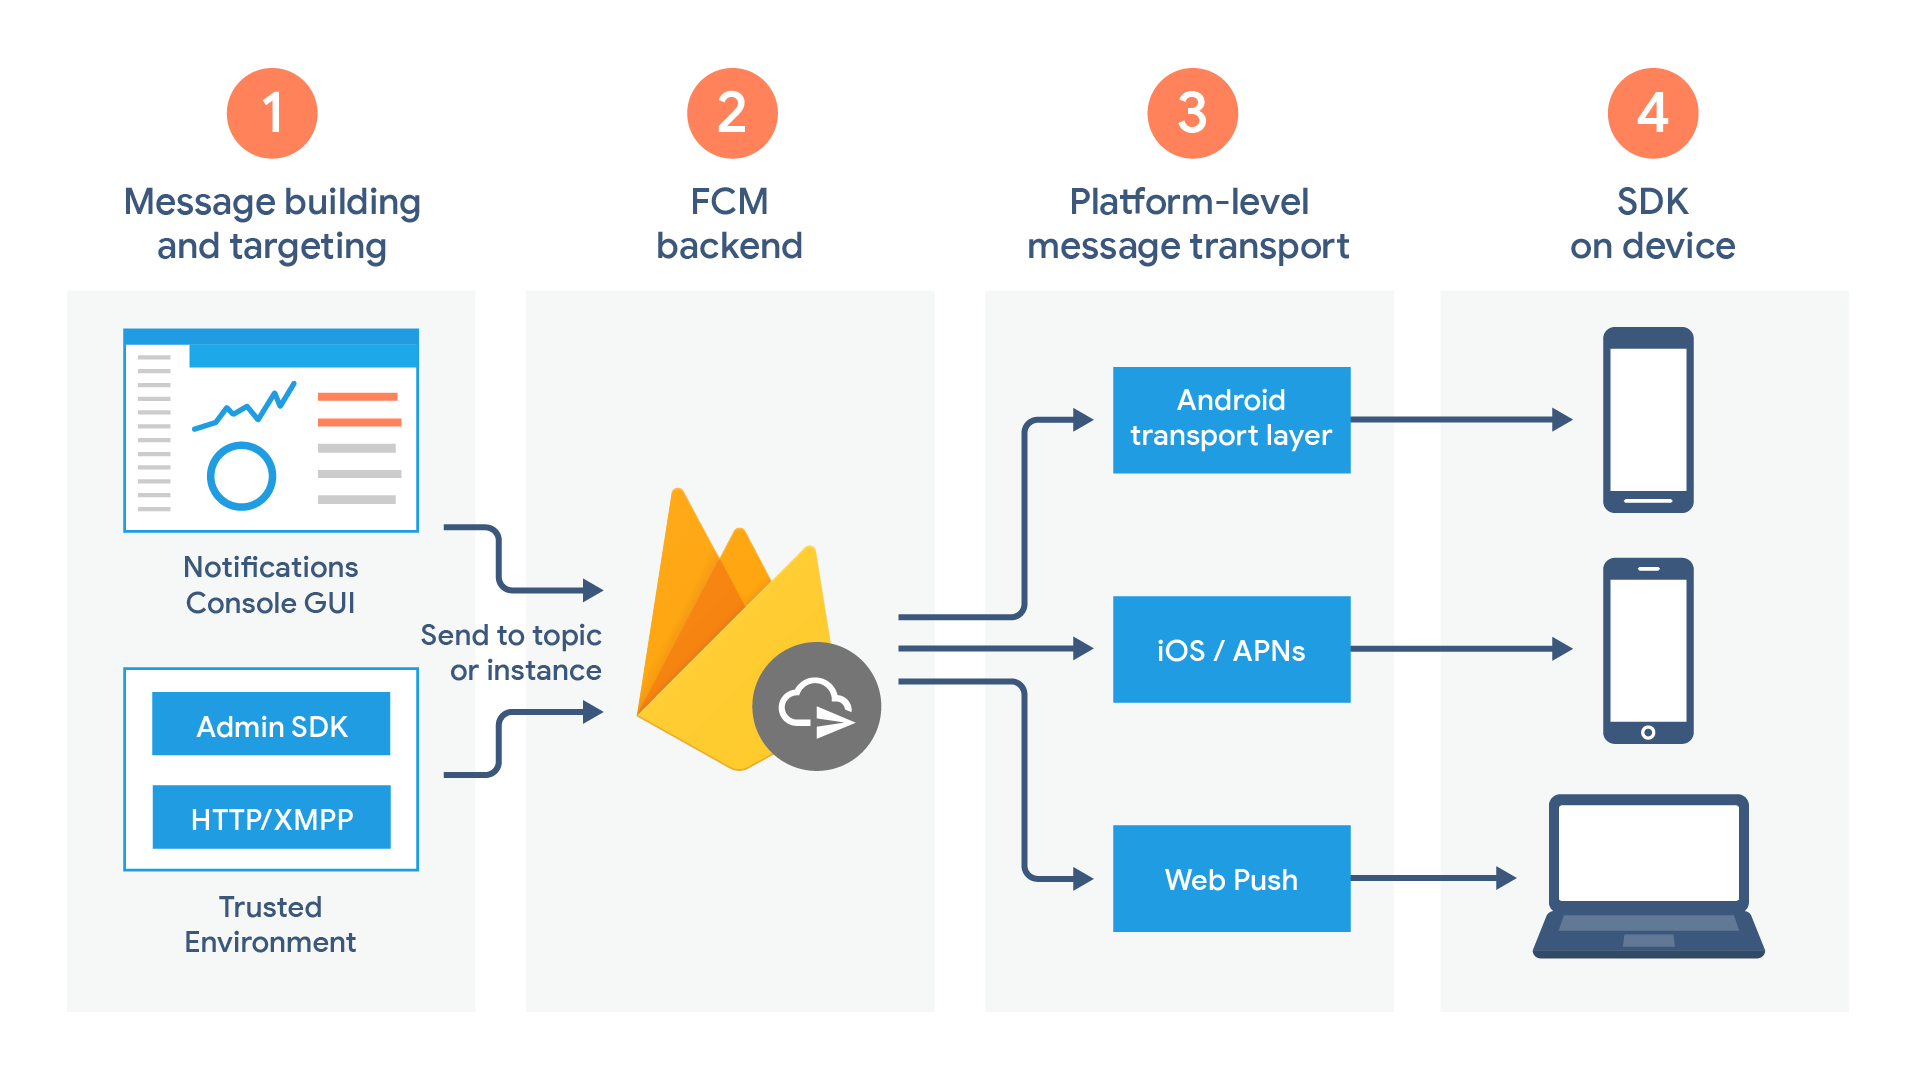
\includegraphics[scale=0.23]{images/firebase_cloudmessaging_architecture.png}
	\end{center}
	\caption{Firebase Cloud Messaging Architektur}
	\label{fig:cloudmessaging_architecture}
\end{figure}

\subsubsection{Google AdMob}
Google AdMob bietet eine einfache Art, gezielte Werbung innerhalb der Anwendung zu schalten und somit die Anwendung zu monetarisieren.
Zusätzlich bietet das Tool in Kombination mit Google Analytics\footnote{Ein freies Analysetool, welches über alle Tools hinweg Ereignisse sammelt und diese Werte direkt graphisch darstellt. Da es für die Implementierung nicht weiter relevant ist, wird es nicht detaillierter besprochen. Zusätzliche Informationen unter \href{https://firebase.google.com/docs/analytics}{firebase.google.com}.} zusätzliche Anwendungsdaten und Analysefähigkeiten.\\
Werbung lässt sich in unterschiedlicher Weise anzeigen (siehe Abbildung \ref{fig:firebase_admob})und lässt sich reibungslos in UI Komponenten integrieren. 
Verschiedene Features sind hier jedoch plattformabhängig. 
Auf der Android Plattform ist es für Nutzer möglich, beworbene Produkte direkt aus der Anwendung heraus zu kaufen.\\
Ein weiteres Werbetool \textit{Google Mobile Ads SDK} ist eine alleinstehende SDK, hingegen Google AdMob bietet einfache Integration in Firebase und weitere Tools.\cite{firebase2021}

\begin{figure}[htb]
	\begin{center}
		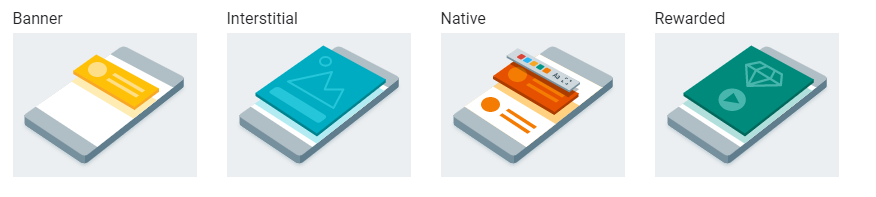
\includegraphics[scale=0.55]{images/firebase_admob_ads.PNG}
	\end{center}
	\caption{Google AdMob Anzeigemöglichkeiten}
	\label{fig:firebase_admob}
\end{figure}






































\subsection{Recommender System}
Auf der Webseite Youtube allein werden minütlich mehr als 500 Stunden Videomaterial hochgeladen. (\url{https://blog.youtube/press/}, 10.02.2021)
Um bei einer solch unvorstellbaren Menge an Daten (allein auf einer Webseite) den Überblick als Endnutzer behalten zu können, ist ein personalisierten Filtersystems unausweichlich.

\noindent
Solche Filtersysteme, auch Recommendation System genannt, nutzt bisher gesammelte Daten um Nutzern potentiell interessante Objekte jeweils individuell vorzuschlagen.
Ein sogenannter \textit{Candidate Generator} ist hierbei ein Recommendation System, welches die Menge $M$ als Eingabe erhält und für jeden Nutzer eine Menge $N$ ausgibt. Hierbei umfasst $M$ alle Objekte und gleichzeitig gilt $N \subset M$. 

\noindent
Die Bestimmung einer solchen Menge $N$ beruht grundlegend auf zwei Informationsarten. Erstens die sogenannten Nutzer-Objekt Interaktionen, also beispielsweise Bewertungen oder auch Verhaltensmuster; Und zweitens die Attributwerte von jeweils Nutzer oder Item, also beispielsweise Vorlieben von Nutzern oder Eigenschaften von Items.\cite{aggarwal2016}
Systeme, welche zum Bewerten ersteres benutzen, werden \textit{collaborative filtering} Modelle genannt. Andere, welche zweiteres verwenden, werden \textit{content-based filtering} Modelle genannt. Wichtig hierbei ist jedoch, dass \textit{content-based filtering} Modelle ebenfalls Nutzer-Objekt Interaktionen (v.a. Bewertungen) verwenden können, jedoch bezieht sich dieses Modell nur auf einzelne Nutzer - \textit{collaborative filtering} basiert auf Verhaltensmustern von allen Nutzern bzw. allen Objekten.

\noindent
Ein solches Recommendation System kann im einfachsten Fall wie in \ref{Recommendation Matrix} als Matrix dargestellt werden.

\begin{table}[tbt]
	\caption{Nutzer-Item Matrix mit Bewertungen. Jede Zelle $r_{u;i}$ steht hierbei für die Bewertung des Nutzers $u$ an der Stelle $i$}
	\centering
	\label{Recommendation Matrix}
	\begin{tabular}{lcllllll}
		& \multicolumn{7}{c}{Items}                                                                                                                                                        \\
		& \multicolumn{1}{l}{}     & \multicolumn{1}{c}{1}  & \multicolumn{1}{c}{2}  & \multicolumn{1}{c}{...} & \multicolumn{1}{c}{i}  & \multicolumn{1}{c}{...} & \multicolumn{1}{c}{m}  \\ \cline{3-8} 
		& \multicolumn{1}{c|}{1}   & \multicolumn{1}{l|}{2} & \multicolumn{1}{l|}{}  & \multicolumn{1}{l|}{1}  & \multicolumn{1}{l|}{}  & \multicolumn{1}{l|}{}   & \multicolumn{1}{l|}{3} \\ \cline{3-8} 
		Users & \multicolumn{1}{c|}{2}   & \multicolumn{1}{l|}{4} & \multicolumn{1}{l|}{}  & \multicolumn{1}{l|}{}   & \multicolumn{1}{l|}{5} & \multicolumn{1}{l|}{}   & \multicolumn{1}{l|}{}  \\ \cline{3-8} 
		& \multicolumn{1}{c|}{...} & \multicolumn{1}{l|}{}  & \multicolumn{1}{l|}{}  & \multicolumn{1}{l|}{1}  & \multicolumn{1}{l|}{}  & \multicolumn{1}{l|}{}   & \multicolumn{1}{l|}{4} \\ \cline{3-8} 
		& \multicolumn{1}{c|}{u}   & \multicolumn{1}{l|}{}  & \multicolumn{1}{l|}{4} & \multicolumn{1}{l|}{}   & \multicolumn{1}{l|}{5} & \multicolumn{1}{l|}{}   & \multicolumn{1}{l|}{1} \\ \cline{3-8} 
		& \multicolumn{1}{l|}{}    & \multicolumn{1}{l|}{2} & \multicolumn{1}{l|}{}  & \multicolumn{1}{l|}{}   & \multicolumn{1}{l|}{}  & \multicolumn{1}{l|}{3}  & \multicolumn{1}{l|}{}  \\ \cline{3-8} 
		& \multicolumn{1}{l|}{n}   & \multicolumn{1}{l|}{}  & \multicolumn{1}{l|}{4} & \multicolumn{1}{l|}{}   & \multicolumn{1}{l|}{3} & \multicolumn{1}{l|}{}   & \multicolumn{1}{l|}{}  \\ \cline{3-8} 
	\end{tabular}
\end{table}

\subsubsection{Nutzerinformation}
Damit ein \textit{Recommender System} einem Nutzer Vorschläge bereitstellen kann, benötigt es Nutzerinformationen. Das Design des jeweiligen Systems hängt auch, wie oben beschrieben, von der Art der Information und von der Art der Beschaffung dieser ab.

\paragraph{Explizite Nutzerinformation}
Bei der expliziten Methode muss der Nutzer individuelle Informationen aktiv über sich preisgeben. Dies kann über konkrete Fragestellungen zu beispielsweise Geburtsdatum, Geschlecht oder Interessen geschehen. Diese Art der Information beschreiben einen Nutzer konkret. 

\noindent
Eine andere Art der Information sind Bewertungen von Objekten. Diese lassen sich beispielsweise Intervall basiert darstellen. Hierbei werden geordnete Zahlen in einem Intervall als Indikator genutzt, ob ein Objekt gut oder schlecht war - zum Beispiel eine Bewertung eines Produktes von 0 bis 5 Sternen bei Amazon. Diese Information beschreiben die Vorlieben eines Nutzers konkret.

\noindent
Je größer diese Skala ist, desto differenzierter ist auch das Meinungsbild, da jeder Nutzer sich genau ausdrücken kann. Jedoch desto komplizierter und unübersichtlich wird auch das Bewertungsverfahren an sich, da man einen zu großen Entscheidungsraum für den Nutzer darbietet.

\paragraph{Implizite Nutzerinformation}
Um implizit Nutzerinformationen zu erfassen, muss ein System die Verhaltensmuster seiner Kunden als Daten abspeichern. Beispielsweise könnte das System von YouTube erfassen, ob Videos frühzeitig abgebrochen oder ganz angeschaut werden. Anklicken von Webseiten und die darauf verbrachte Zeit könnte ebenfalls als Bewertung gespeichert und zur Generierung von Vorschlägen genutzt werden.

\subsubsection{Content-based filtering}
Unter \textit{content-based filtering} versteht man das Betrachten von Ähnlichkeiten zwischen Objekten anhand von Schlüsselwörtern (Eigenschaften) und daraus dann das Vorhersagen der Nutzer-Objekt Kombination für ein bestimmtes Objekt. 
Nimmt man an, Film 1 und Film 2 haben ähnliche Eigenschaften (gleiches Genre, gleiche Schauspieler, ...) und Nutzer A mag Film 1, so wird das System Film 2 vorschlagen.

\noindent
Das System ist also unabhängig von anderen Nutzerdaten, da die Vorschläge nur auf Präferenzen eines einzelnen Nutzers basieren. Dies bietet im Hinblick auf eine App auch gute Skalierungs"-möglich"-keiten. Zudem kann auf Nischen-Präferenzen gut eingegangen werden, da nicht mit anderen Nutzerdaten verglichen wird, sondern nur ein Nutzer für sich betrachtet wird.

\noindent
Gleichzeitig schlagen \textit{content-based filtering} Systeme aber eher offensichtliche Objekte vor, da Nutzer oft unzureichend genaue "Beschreibungen", also Vorlieben mit sich bringen. Dadurch, dass nur basierend auf Schlüsselwörter neue Objekte vorgeschlagen und andere Nutzerwertungen nicht miteinbezogen werden, sind die Vorschläge sehr wahrscheinlich oftmals ähnlich bis gleich - man "verfängt" sich quasi in eine Richtung.\cite{aggarwal2016}

\subsubsection{Collaborative Filtering}
Unter \textit{collaborative filtering} versteht man das Betrachten von Ähnlichkeiten im Verhalten von Nutzern anhand von Bewertungen und Prä"-fer"-enzen, bzw. anhand der Ähn"-lich"-keiten von Objekten.

\noindent
Generell unterscheidet man in zwei Typen:\cite{aggarwal2016}

\begin{enumerate}		
	\item \textit{Memory-based Methoden}: Es wird, wie oben beschrieben, aus gesammelten Daten Ähn"-lich"-keit herausgearbeitet und Nutzer-Objekt Kombinationen durch eben diese vorhergesagt. Daher wird dieser Typ auch \textit{neighborhood-based collaborative filtering} genannt. Man unterscheidet weiter in:
	\begin{enumerate}
		\item \textit{User-based}: Ausgehend von einem Nutzer A werden andere Nutzer mit ähnlichen Nutzer-Objekt Kombinationen gesucht, um Vorhersagen für Bewertungen von A zu treffen. Ähnlichkeitsbeziehungen werden also über die Reihen der Bewertungsmatrix berechnet.
		\item \textit{Item-based}: Hierbei werden ähnliche Objekte gesucht und diese genutzt um die Bewertung eines Nutzers für ein Objekt vorherzusagen. Es werden somit Spalten für die Berechnung der Ähnlichkeitsbeziehungen verwendet.
	\end{enumerate}
	\item \textit{Model-based Methoden}: Machine Learning und Data Mining Methoden werden verwendet um Vorhersagen über Nutzer-Objekt Kombinationen zu treffen. Hierbei sind auch gute Vorhersagen bei niedriger Bewertungsdichte in der Matrix möglich.
\end{enumerate}

\noindent
Vereinfacht gesagt: Wenn Nutzer A ähnliche Bewertungen verteilt wie Nutzer B, und B den Film 1 positiv bewertet hat, wird das System Film 1 auch Nutzer A vorschlagen. Das selbe gilt auch umgekehrt (\textit{Item-based}).

\noindent
Diese Art leidet sehr unter dem \textit{sparsity} Problem, also dass die Nutzer zu wenige Bewertungen von Objekten ausüben. Daher sind Vorhersagen über Ähnlichkeit von Nutzern aufgrund unzureichender Datensätze nicht sinnvoll möglich. Dieses Problem wird \textit{Cold-Start Problem} genannt.

\subsubsection{Ähnlichkeit von Objekten und Nutzern}
Sowohl bei \textit{collaborative filtering}, als auch bei \textit{content-based filtering} wird jedes Objekt und jeder Nutzer als ein Vektor im Vektorraum-Modell $E = \mathbb{R}^d$ (englisch \textit{embedding space}) erfasst. Sind Objekte beispielsweise ähnlich, haben sie eine geringe Distanz voneinander. 

\noindent
Ähnlichkeitsfunktionen sind Funktionen $s : E \times E  \rightarrow \mathbb{R}$ welche aus zwei Vektoren beispielsweise von einem Objekt $q \in E$ und einem Nutzer $x \in E$ ein Skalar berechnen, welches die Ähnlichkeit dieser zwei beschreibt $s(q,x)$.

\noindent
Hierfür werden mindestens eine der folgenden Funktionen verwendet:
\begin{itemize}
	\item Cosinus-Funktion
	\item Skalarprodukt
	\item Euklidischer Abstand
\end{itemize} 

\paragraph{Cosinus-Funktion}
Hier wird einfach der Winkel zwischen beiden Vektoren berechnet: $s(q,x) = \cos(q,x)$

\paragraph{Skalarprodukt}
Je größer das Skalarprodukt, desto ähnlicher sind sich die Vektoren. $s(q,x) = q \circ x = \sum_{i=1}^{d}q_i x_i$ 

\paragraph{Euklidischer Abstand}
$s(q,x) = ||q-x|| = [\sum_{i=1}^{d}(q_i - x_i)^2]^\frac{1}{2}$





\url{https://dl.acm.org/doi/pdf/10.1145/3383313.3412488}
\url{http://www.microlinkcolleges.net/elib/files/undergraduate/Photography/504703.pdf}	
		
\section{Konzept?}

		

\section{Funktionen/Komponenten}

\subsection{Swipe/Aussuchen/Voting}		
\subsection{Matches/Chat}		
\subsection{Film-/Serienvorschläge}		
\subsection{Gruppenorgien}		
\subsection{Gespeicherte Filme/Filmliste}		
\subsection{Zugänglichkeit/Behindertenfreundlichkeit}		


\section{Benutzeroberflächen}
\subsection{Home-Screen}
\subsection{Gruppen}		
\subsection{Chat}		
\subsection{Filmliste}

\section{CodeBeispiele}


\section{Probleme}


\section{Fazit}
\section*{Literaturverzeichnis}
\begin{itemize}
	\bibitem[1]{aggarwal2016} Aggarwal, C. C. (2016). Recommender systems (Vol. 1). Cham: Springer International Publishing.
	\bibitem[2]{fentaw2020} Fentaw A. E. (2020). Cross platform mobile application development: a comparison study
	of React Native Vs Flutter.
	\bibitem[3]{flutter2021} Flutter Flutter architectural overview [Online] Verfügbar: \url{https://flutter.dev/docs/resources/architectural-overview}, Aufgerufen am: 04.03.2021
	\bibitem[4]{cisco2020} Cisco (2020) Cisco Annual Internet Report (2018–2023) White Paper [Online] Verfügbar: \url{https://www.cisco.com/c/en/us/solutions/collateral/executive-perspectives/annual-internet-report/white-paper-c11-741490.html}
	
\end{itemize}

\end{document}




%************************************************************%
%*********************End of document************************%
%************************************************************%

\footnote{\url{https://de.wikipedia.org/wiki/Alufolie}} 


Abbildung \ref{fig:allg_kennlinie}

\begin{figure}[tbt]
\begin{center}
\includegraphics[scale=0.45]{Grafiken/allg_kennlinie.png}
\end{center}
\caption{Kennlinie einer Halbleiterdiode \protect \footnotemark}
\label{fig:allg_kennlinie}
\end{figure}
\footnotetext{FUSSNOTE}


Tabelle \ref{tab:cobalt}

\begin{table}[tbt]
\caption{•}
\begin{threeparttable}	%Scheme for footnotes in tables
\begin{center}
\begin{tabular}{c c c c}
\toprule
& keV & keV & keV \\
\midrule
a	& b	& c	& d \\
a	& b	& c	& d \\
a	& b	& c	& d \\
a	& b	& c	& d \\ %direkt hinter jeweiligen Wert /tnote{1}
\bottomrule
\end{tabular}
\end{center}
\begin{tablenotes}\footnotesize 
\item[1]{Quelle: http://www.thinksrs.com/downloads/PDFs/ApplicationNotes/IG1BAgasapp.pdf}
\end{tablenotes}
\end{threeparttable}
\label{tab:cobalt}
\end{table}